\section{Deep Learning}
Neural networks are heavily researched for numerous applications and they are loosely
based on the way a brain functions. The basic model a \ac{nn} consist of inputs, outputs
and a connecting layer of neurons. The use and complexity of neural networks have greatly
increased in the recent years as the massively parallel architecture of GPUs has been
used to gain significant increases in speed compared to what is possible on CPU based
implementations~\cite{NIPS_IMAGENET}. This chapter introduces the basic concepts behind
general deep neural networks, convolutional neural networks and stacked denoising
autoencoders.~\ref{ssec:dldnn} and~\ref{ssec:dlcnn} are based on the book Deep Learning
by Goodfellow et.~al.~\cite{DEEP_LEARNING}.

\subsection{Deep neural networks}\label{ssec:dldnn}

A \ac{dnn} is commonly defined as a \ac{nn} that has a visible input and output layer
with several hidden layers between them. The distinction between visible and hidden
layers is important because training of the network only evaluates the output layer's
performance. During training, a learning algorithm optimizes the individual hidden
layers to best approximate the desired output of the whole network.

The input layer takes in the data to be processed, which typically means a vector of
color values in the case of object tracking. These are then processed by the hidden
layers and finally the output layer produces the target's position in the frame. These
models usually come in the form of a feedforward neural network or \ac{mlp}. The name
comes from the fact that information flows from the input through computations to the
output with no feedback connections. Typically, this means that connections are only
between consecutive layers.

In \ac{nn}s, each layer consists of several units with an activation function and a
weight for each of their input connections. The weights of the layer's inputs are
commonly represented by a matrix by which the input vector is multiplied as each row
represents a unit's input weights. All units can be connected to all inputs (fig.\ref{fig:fcon})
forming a fully connected layer or just some of them (fig.\ref{fig:scon}) utilizing
sparse connections. Sparse layers can be implemented by defining unique input vectors
for the units. Units in a layer have a common activation function that is fed by the
sum of its weighted inputs. The \ac{relu} is a commonly used unit type and is defined
by the activation function $g (z) = \max\{0,z\}$. It provides a nonlinear transformation
while being comparable to linear models in terms of generalizing well and being easy to
optimize. A bias-term can also be defined for each unit and a vector containing the layer's
biases is summed to the outputs of the activation function before passing the results to
the next layer.

\begin{figure}[H]
\centering
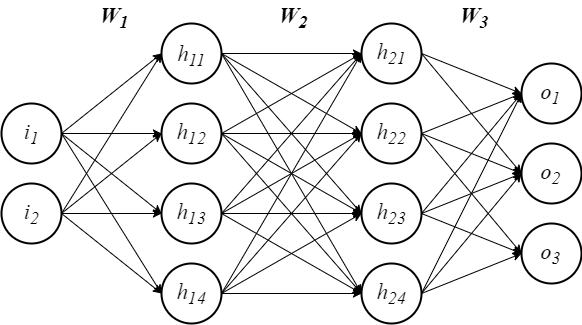
\includegraphics[width=0.75\textwidth]{dnn}
\caption{A fully connected network with two inputs \textit{i}, two hidden layers of
         four units \textit{h} and three outputs \textit{o}. Each set of connections
         is represented by a weight matrix \textbf{W} which indicates mapping from one
         layer to another. Excluding the input, all layers also have an activation
         function and their units can be assigned individual weights.}\label{fig:fcon}
\end{figure}

Before training, the weights of a \ac{mlp} are initialized to small random values and
biases to zero or small positive values. Then an algorithm called stochastic gradient
descent is commonly applied alongside a training dataset. The basic procedure is to
calculate the error of the network's output values compared to the desired ones using
a loss function. The function's gradient can then be calculated for example by back-propagation,
which feeds the errors back through the network to assign a contribution value to each unit.
These values are then used to calculate the gradient of the loss function relative to the
weights. Each weight is adjusted slightly to the opposite sign to minimize the loss function.

\subsection{Convolutional neural networks}\label{ssec:dlcnn}

``Convolutional networks are simply neural networks that use convolution in place of
general matrix multiplication in at least one of their layers''~\cite{DEEP_LEARNING}.
Intuitively, convolution can be viewed as a blending of two functions as it is an
integral expressing the overlap of two functions as one is moved over the other.
A convolution performed on integers is by definition an infinite summation but it
can be implemented on a finite number of elements if the functions are considered
zero for all values that are not stored. In a \ac{cnn}, a convolution defined by this
property is performed on the input data and a kernel in the form of a vector of weights
learned in training.

A typical convolutional layer consists of three stages: a convolution stage, detector
stage and pooling stage. These operations can be implemented by individual layers. First,
the multiplication of the kernel and the input data is performed in positions separated by
a step size. The result is then fed to a linear activation function. In the detector stage,
the results are then run through a non-linear activation, for example a \ac{relu}. Finally,
a pooling function is used to combine the results of multiple nearby activations as the
final output.

The main motivations in using \ac{cnn}s are sparse interactions, parameter sharing
and equivariant interactions. Units in traditional layers are connected to the whole
input so an input sized \textit{m} and output of size \textit{n} form a computational
complexity of $m \times n$. Convolutional layers' units typically only connect to a small
portion of the input, which can be a significant decrease in computation: a kernel of
size \textit{k} results in a complexity $k \times n$ and \textit{k} can be kept several
orders of magnitude smaller than \textit{m}. It is also possible to share the same kernel
for all positions in the input to reduce the number of weights stored from $m \times n$
to just \textit{k}. Parameter sharing in convolution also results in equivariance to
translation. It is a useful property in processing 2D data as a shift in the input
results in a similar shift in the output. Equivariance to some other transformations is not
inherent to convolution so other mechanisms are required for handling them.

\begin{figure}[H]
\centering
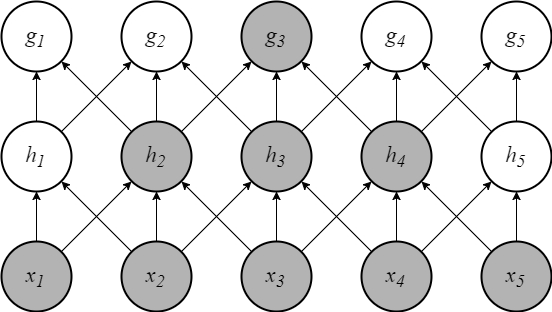
\includegraphics[width=0.75\textwidth]{cnn}
\caption{Stacking convolutions can provide deeper layers indirect connections to
         most or all of the input data even though their direct connections are sparse.
         This forms hierarchies of features that are useful for capturing larger concepts
         and the effect increases if a strided convolution or pooling is used.~\cite{DEEP_LEARNING}
         Source: Recreated fig. 9.4 from Deep Learing~\cite{DEEP_LEARNING}}\label{fig:scon}
\end{figure}

\begin{figure}[H]
\centering
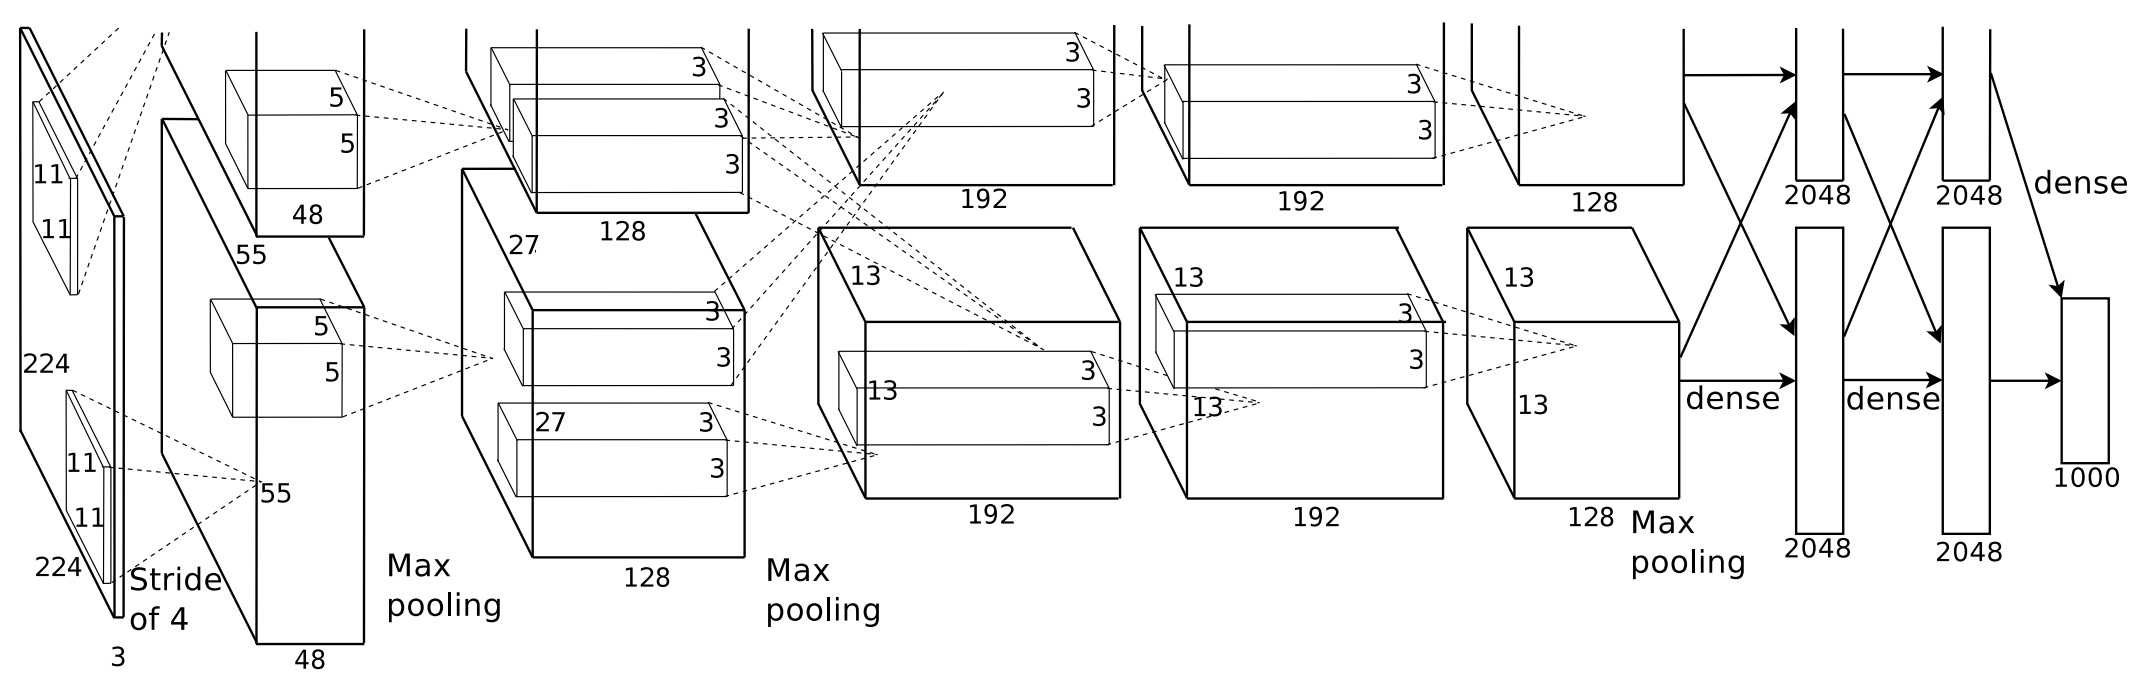
\includegraphics[width=1\textwidth]{cnn2}
\caption{A branch in the network of Krizhevsky et.~al.~\cite{NIPS_IMAGENET} is a good example
         of a basic \ac{cnn} architecture. The first layer uses a 11$\times$11$\times$55
         kernel and feeds into layers of increasing depth with the final convolutional layer
         working with a 3$\times$3$\times$192 kernel. The final layers are fully connected
         and produce the networks output as a vector of probabilities over the 1000 trained
         subject classes. Source: Krizhevsky et.~al.~page 5~\cite{NIPS_IMAGENET}}\label{fig:cnn}
\end{figure}

\subsection{Stacked denoising autoencoders}
Autoencoders consist of an encoder, a decoder and a loss function. They first encode the
given data to a hidden representation and then reconstruct it. The loss function is
used in training to guide the result towards the desired output. Reconstructing the
exact input data is not useful and denoising autoencoders avoid that by learning to
encode a corrupted version of the input and decode the result into useful features of
the clean input. A stacked denoising autoencoder utilizes a sequence of encoders each
encoding the input further with the final encoder feeding a series of matching decoders.
Corrupted input data is only used in training the autoencoder to find useful features as
a trained \ac{sdae} works on clean input.~\cite{SDAE} The encoder halves of \ac{sdae}s
were used for extracting features from tracking sequences especially before research was
done on shift-variant \ac{cnn}s.
